\begin{abstract}
云原生系统日益依赖服务网格、监控智能体等基础设施服务；这些服务会与用户应用争用资源，进而损害性能与可扩展性。本文提出 \xpod：一种把此类服务卸载到数据处理单元（DPU）的新抽象，以实施严格隔离，同时减少主机资源争用与运维成本。为实现 \xpod，本文引入跨处理单元（XPU）网络系统 \os，其包含两项关键能力：（1）\emph{拆分网络命名空间}，为横跨 CPU 与 DPU 的进程提供统一网络抽象；（2）\emph{弹性高效的 XPU 网络}，在不引入固定资源开销和轮询成本的前提下达到共享内存性能。借助 \os 以及云原生工作负载的组合式特征，\xpod 能够以合适方式把基础设施容器卸载到 DPU。我们基于 Linux 实现 \os，并基于 Kubernetes 实现云原生系统 \sys。我们使用 NVIDIA BlueField-2 DPU 和基于 CXL 的 DPU（以真实 CXL 内存设备模拟）评估这些系统。结果表明，\sys 能有效支持复杂且未经修改的通用云原生应用（代码规模最高达 100 万行）；与内核旁路设计相比，其延迟最高改善 $31.9\times$、资源消耗最多降低 $64\times$；与现有先进系统相比，其端到端延迟最多改善 60\%，可扩展性最高提升 55\%。
\end{abstract}

\section{引言}
\label{s:intro}

云原生计算已经成为云和数据中心环境中的重要范式，它利用\emph{容器化}来分发和部署应用\cite{cncf,AWSLambda,IBMcloudFn,MSFunc,GoogleFunc}。执行环境的基本单元，例如 Kubernetes 中的 \emph{Pod}\footnote{本文把 Pod 视为云原生平台基本计算单元的广义表示。}，通常包含一个或多个容器；每个容器拥有独立镜像，但共享网络环境。借助这种方式，应用被封装成可移植、自包含的单元，并可部署和分发到不同节点。

相较非云原生应用，云原生应用的一项重要优势是其开发过程得到大量云基础设施服务的支持，包括存储、网络与安全等。这些基础设施服务同样以容器部署。基础设施容器可分为两类：全局基础设施容器和逐 Pod 基础设施容器，如图~\ref{fig:motiv-cloud-native-platform}(a) 所示。例如，平台调度器是一种全局基础设施容器，负责把请求编排到不同 Pod；边车代理（如 Envoy\cite{envoy}）则是一种存在于每个 Pod 中的逐 Pod 基础设施容器，为应用提供网络功能。

\begin{figure}[t]
  \centering
  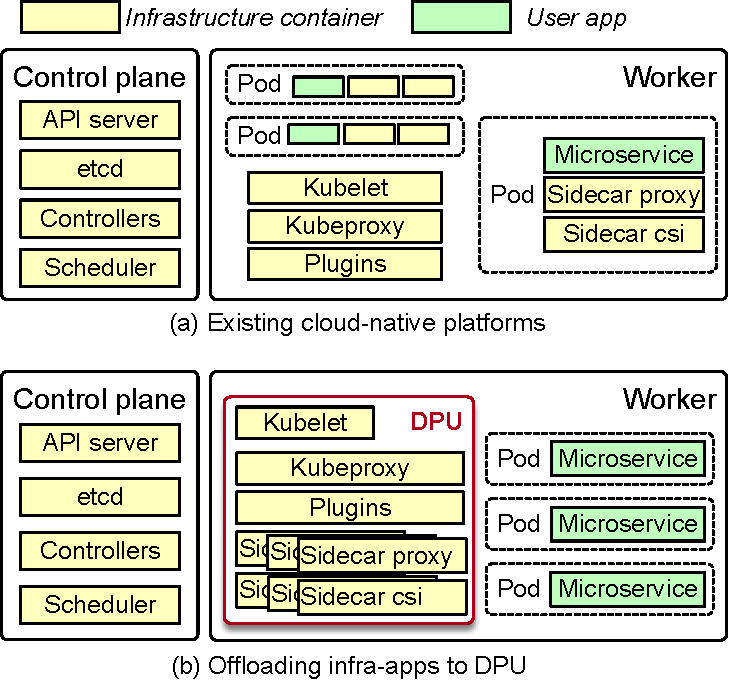
\includegraphics[width=0.98\linewidth]{figs/motiv-cloud-native-platform-eps-converted-to.pdf}
  \caption{包含基础设施容器和用户应用的云原生平台。}
  \label{fig:motiv-cloud-native-platform}
\end{figure}

基础设施容器虽然对发挥云原生计算优势至关重要，却也带来不可忽视的资源负担，本文称之为\emph{基础设施负担（infra-burden）}。例如，服务网格\cite{service-mesh}已经成为云原生平台管理微服务的一种常见模式，它使用专用代理（称为\emph{边车代理}）代替应用处理网络流量。由于每个微服务 Pod 都包含一个作为基础设施容器的边车代理，这些代理容器可能消耗节点上最高 25\% 的 CPU 和 33\% 的内存资源\cite{10.1145/3620678.3624785}。基础设施负担问题已持续很长时间\cite{10.1145/3477132.3483565}，而且非常难以缓解\cite{10.1145/3694715.3695967,10.1145/3694715.3695947,10.1145/3694715.3695966}。

近期一个可能带来缓解的重要趋势是，\emph{云厂商正在部署越来越多的异构设备}，以提高可扩展性、性能与成本效率\cite{amazon-f1,silberstein2013gpufs,kim2014gpunet,firestone2018azure,china-mobile-smartnic,huawei-smartnic,xilinx-fpga-huawei,ali-fpga,baidu-fpga}。数据处理单元（DPU）是一类新型异构设备，它通过嵌入式处理单元和高效 NIC 提供可扩展、节能的计算能力\cite{234944}。DPU 有望显著提高单节点的实例密度，例如在无服务器计算中提升 50\%\cite{10.1145/3503222.3507732}。隔离的内存和核心还为这些设备提供了更强的安全性，而大量位于数据路径上的硬件线程可提升分组处理能力；例如 BlueField-3 支持 256 个硬件线程\cite{bf-3}。预期 DPU 等异构处理单元将通过 PCIe 6.0、CXL\cite{intel-cxl} 等高速互连连接，从而进一步提升性能。利用 DPU 因而可能缓解基础设施负担。

\myparagraph{目标：把云原生基础设施服务卸载到 DPU。}
传统方法会在 CPU 和 DPU 上共同放置基础设施容器与用户应用\cite{redhat-openshift}；与之不同，我们提出一种很有潜力但也颇具挑战的体系结构：把这两类云原生容器解耦到不同处理单元（PU），如图~\ref{fig:motiv-cloud-native-platform}(b) 所示。该策略通过避免基础设施容器和应用容器相互干扰，可以有效缓解基础设施负担。然而，把基础设施容器与应用容器分开也带来显著挑战。

\myparagraph{挑战 1：同一 Pod 中的基础设施容器与应用容器耦合在同一个网络命名空间中，并依赖单 PU 操作系统。}
共享 Pod 内的容器使用底层操作系统内核提供的网络命名空间。因此，不同容器中的进程共享网络设备，并可使用 ``localhost'' 进行跨容器通信。把基础设施容器卸载到 DPU 会破坏这种共享网络命名空间能力。在把基础设施容器和应用容器分布到不同 PU 的同时保持本地网络抽象，是一个突出难题。

\myparagraph{挑战 2：把容器拆分到不同 PU 会在通信性能与资源利用率之间形成权衡。}
基础设施容器与应用容器将通过网络通信。由于网络分组需要经过两个 NIC，相较采用 Linux 网络栈的单 PU 设计，这种拆分可能使通信延迟增加 $10\times$ 到 $100\times$。rsocket\cite{rsocket} 等内核旁路机制\cite{10.5555/2616448.2616493,rsocket,f-stack,10.1145/3341302.3342071,libvma}可以提供兼容的套接字级 API，并直接利用 RDMA 等硬件能力获得理想性能。然而，这些方案往往面临资源利用不佳的问题\cite{10.1145/3477132.3483569}，包括为用户态链路分配固定内存造成的浪费，以及用户态轮询浪费的 CPU 周期。SMC-R\cite{rfc7609} 等内核辅助方法则受上下文切换和数据复制开销影响。因此，系统迫切需要一种跨 PU、基于网络的通信方式，在提供高性能的同时最大化资源利用率；当前尚无这样的方案。

\myparagraph{挑战 3：并非所有基础设施容器都适合卸载到 DPU。}
这一挑战源于 DPU 的固有特征：DPU 通常只包含面向特定领域任务（如网络分组处理）优化的低性能 SoC。既有研究表明，直接把容器卸载到 DPU 的简单设计可能带来显著性能开销\cite{wei2022comprehensive,10.1145/3477132.3483565,10.1145/3503222.3507732}。因此，系统设计者仍缺少有效卸载云原生基础设施的实践方法。

本文提出跨 PU Pod 设计 \xpod，并以 \os 解决前两个挑战，实现透明、高性能且资源高效的 XPU 网络。\os 引入两项关键技术：\emph{拆分网络命名空间}（\giptable）和\emph{弹性高效的 XPU 网络}（\gsocket）。\giptable 为跨 PU 容器提供统一网络抽象；其新意在于通过在多个 PU 上\emph{重新执行}网络规则来建立拆分网络命名空间，使直接和间接通信都能照常进行。其次，\gsocket 是一种同时达到内核旁路性能、高资源效率和套接字兼容性的网络栈。\gsocket 采用\emph{推测式分配}来缓解内存浪费：其两阶段按需缓冲区分配允许进程以绕过内核的方式从共享池中推测式申请新缓冲区，之后再由内核提交该分配。此外，\gsocket 支持用户态 NAPI 和跨 PU 操作系统协作，利用页表与异常为用户态库提供中断能力，从而降低轮询成本。

我们利用 \xpod 实现了基于 Kubernetes 的云原生系统 \sys；该系统支持无服务器计算（\faas）和带服务网格的微服务（\mesh\cite{istio}）。\sys 可以有效卸载边车代理等逐 Pod 基础设施容器和调度器等全局基础设施容器，同时也足够通用，能够卸载无服务器场景中合适的用户应用以提高系统密度。因此，\sys 也为第三个挑战提供了卸载基础设施容器的实践准则。

我们在配有 NVIDIA BlueField-2 DPU 的真实平台和基于真实 CXL 内存设备构建的 CXL-DPU 模拟平台上评估全部原型。结果表明，\gsocket 的延迟最高改善 $31.9\times$，资源消耗最多降低 $64\times$。与商用 Istio 相比，\mesh 的可扩展性最高提升 55\%，端到端延迟最多改善 60\%；与基线系统相比，\faas 的通信延迟最高降低 $20\times$，应用延迟最高降低 $4.45\times$。\sys 还能把控制面调度器卸载到 DPU，在那里缓存全局镜像状态并实现镜像感知调度，使平均延迟降低 $14.4\times$。

\section{动机}
\label{s:challenge}

\subsection{云原生应用及其问题}

云原生应用通常部署在 \emph{Pod} 中；Pod 是 Kubernetes 等平台采用的多容器抽象。如图~\ref{fig:motiv-cloud-native-platform}(a) 所示，我们把云原生\emph{容器}分为基础设施容器和用户容器两类。相较非云原生应用，云原生应用的一项潜在优势在于，\emph{其开发得到庞大的云基础设施服务支持}，包括存储、网络和安全等。例如，云厂商通常为每个微服务（用户容器）部署 Envoy\cite{envoy} 作为基础设施容器，以管理网络。我们强调当今这种云原生体系结构中的两个问题（\textbf{I}）。

\myparagraph{I1：基础设施容器给 CPU 和内存带来显著负担。}
基础设施容器首先会引入不可忽视的资源负担。例如，服务网格\cite{service-mesh}使用专用的\emph{边车代理}代表应用处理网络流量，是管理微服务的一种常用模式（图~\ref{fig:motiv-cloud-native-platform}(a)）。我们用 emoji-voting\cite{emojivote} 微服务评估 Kubernetes 上边车容器引入的资源成本（详细设置见第~\ref{s:case-mesh} 节）。结果显示，代理容器可能消耗节点上最高 25\% 的 CPU 和 33\% 的内存资源。此外，即使 RPS 很低（RPS=20），代理容器仍可能消耗大量资源，进一步加剧节点中的资源干扰。

\myparagraph{I2：对模块化云原生应用而言，通信延迟更加重要。}
微服务和无服务器函数都是细粒度、模块化应用：一个应用可能被划分为几十乃至数千个微服务或函数，它们依赖通信机制进行协作。由于每项服务的执行时间只有几毫秒，通信延迟对端到端性能十分重要。事实上，边车代理等基础设施容器甚至会进一步增加延迟：使用代理 Envoy 后，延迟可能增加 $9.5\times$（RPS=20）到 $49.8\times$（RPS=3K）\cite{10.1145/3620678.3624785}。为了规避这项成本，目前常见的做法是把一条函数链（或高度相关的微服务）部署在同一节点，并依靠 IPC 或域套接字等本地通信方法降低延迟\cite{jianightcore,10.1145/3503222.3507732,273833,akkus2018sand}。这导出一项重要要求：\emph{提高用户应用密度，而且越高越好}。但基础设施容器的干扰使这一目标很难实现。

\begin{figure}[t]
  \centering
  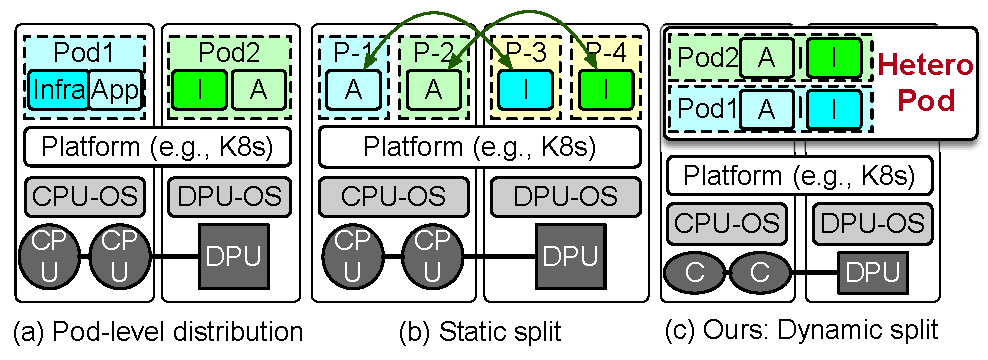
\includegraphics[width=0.98\linewidth]{figs/intro-cloud-native-issue-eps-converted-to.pdf}
  \caption{CPU--DPU 计算机上的云原生应用。}
  \label{fig:intro-issue}
\end{figure}

\subsection{面向云原生应用的 CPU--DPU 平台}
\label{s:dpu}

DPU（数据处理单元）\cite{netronomeagilio,mellanoxbf,marvel-octeon-sdk}是一类在数据中心内移动和处理数据的新型可编程设备。DPU 是能够运行商用操作系统以及网络代理等性能关键程序的 SoC，通常包含多核处理单元（例如 BlueField-2 DPU 中 2.75GHz 的 ARM 核心）和高效网络接口。既有工作已经证明，DPU 可以提高无服务器函数密度\cite{10.1145/3503222.3507732}、降低分布式文件系统的延迟和资源成本\cite{10.1145/3477132.3483565}，并实现节能微服务\cite{234944}。

\myparagraph{将 DPU 用于云原生应用的既有尝试。}
如图~\ref{fig:intro-issue}(a)(b) 所示，商用云平台通常采用\emph{Pod 级分布}，例如 NVIDIA DPU Container\cite{nvidia-doca-container} 和 Red Hat OpenShift\cite{redhat-openshift}；或者采用\emph{静态拆分}\cite{10.1145/3477132.3483565,li2020leapio,seshadri2014willow}，例如 Azure\cite{firestone2018azure}。Pod 级分布把 DPU 当作独立服务器，直接在 DPU 上部署未经修改的应用。然而，应用需求与硬件能力可能不匹配，例如 DPU 往往只有低性能核心，因而应用可能出现显著性能下降。静态拆分则把应用拆成细粒度组件并分发到不同 PU，通过通信协作；它只把适合的组件部署到 DPU，例如让 CPU 运行计算密集组件、DPU 运行网络密集组件，因而能取得良好性能。但这种方法通常要求在开发阶段理解应用和硬件，难以适配通用应用与多样的异构设备。尽管如此，两类方法在真实工业应用中都具有实用性，并能提供特定收益。

近期研究针对无服务器计算\cite{10.1145/3503222.3507732}、微服务\cite{234944}等特定云原生场景开发了新的异构框架。然而，这些框架通常要求修改应用，因此只能支持简单应用（例如 Molecule\cite{10.1145/3503222.3507732}只支持少于 1.8K 行 Node.js 代码），对于 Envoy 这类复杂通用应用则\emph{不够实用}；Envoy 是广泛使用的服务网格代理，包含 764K 行 C++ 代码。许多通用云原生应用以二进制或容器镜像形式分发，很难修改，因此上述限制尤为显著。

\myparagraph{本文方法：使用 \xpod 动态拆分。}
与既有方法不同，我们提出\emph{动态跨 PU 解耦}：在运行时透明地把容器（即使属于同一 Pod）划分到不同异构 PU，如图~\ref{fig:intro-issue}(c) 所示。我们把这种体系结构称为 \xpod（跨 PU Pod），它解决了传统部署中的关键局限。第一，把基础设施容器隔离到 DPU 可以消除其与应用容器的资源争用。第二，把合适的用户容器也卸载到 DPU，可帮助提高单节点密度。第三，也是最重要的一点，与静态拆分不同，\xpod 的动态拆分保留现有 Pod 语义，因此能支持未经修改的通用云原生应用。

\section{\xpod 设计概览}
\label{s:design-overview}

\xpod 的核心思想很简单：选择性地把基础设施容器和应用容器部署到 DPU，其余容器继续留在 CPU 上。这种容器粒度部署利用每个容器的自包含特征简化解耦。不过，关键挑战在于\textbf{跨容器通信}，因为云原生平台中的容器依赖网络交互。

具体而言，\xpod 必须解决两项技术挑战：（1）提供透明的跨 PU 网络，从而支持未经修改的应用，即第~\ref{s:intro} 节的\textbf{挑战 1}；（2）实现高效率的跨 PU 通信，即第~\ref{s:intro} 节的\textbf{挑战 2}。为此，我们把 \os 设计为 \xpod 的基础技术；\os 为跨 PU（XPU）网络引入两项关键创新。

第一，\os 实现 \giptable，为跨 PU 容器提供统一网络抽象。\giptable 以全局端口空间为指示器来支持跨 PU 直接连接，并利用如下观察支持跨 PU 间接通信：只要不引入新的副作用，网络过滤器或规则就可冗余地应用于源 PU 和目标 PU。由此，\giptable 创建一个拆分网络命名空间，在不同 PU 的组件之间保留通信语义。第二，\os 引入 \gsocket，这是一种内核与库协同设计的网络栈，同时实现内核旁路性能、内核辅助的资源效率和套接字 API 兼容性。\gsocket 采用两项关键机制：\emph{推测式分配}是一种两阶段缓冲区管理策略，进程先从共享池临时领取缓冲区（绕过内核），再由内核验证并提交分配；\emph{用户态 NAPI}利用跨 PU 操作系统协作，使用户态库可以通过中断驱动处理事件，从而显著减少轮询开销。
